\section{Introducción}
El objetivo es ordenar hasta cien empresas por su probabilidad de ganar una licitación usando únicamente información previa a su publicación. El modelo de referencia B0 estima esa probabilidad a partir de adjudicaciones anteriores, ponderadas por antigüedad y coincidencia en oficina, tipo de compra (PSC), actividad económica (NAICS) y modalidad de reserva. Sin embargo, en el 68--84\,\% de las licitaciones, según el rubro, no sitúa a ningún ganador entre las diez primeras empresas. Se busca determinar cuánto aportan el texto y otras relaciones observables, mediante un modelo interpretable y compartido entre rubros.

\section{Modelo y datos}
Se analizaron cinco rubros: IT y telecomunicaciones (d), productos informáticos (it), mantenimiento (j), servicios profesionales (r) e investigación y desarrollo (rd). Cada licitación tiene decenas de miles de candidatas. Para reducir el costo, se construye un \emph{pool} con la unión de las primeras 300 empresas según B0, TF-IDF, título, contrato previo más parecido y difusión; también ingresan las empresas mencionadas por su nombre en el aviso. Las pistas restantes se calculan sobre ese conjunto. Se entrena con 2022S2--2023S2, se seleccionan parámetros en validaciones temporales 2023S1 y 2023S2, y se evalúa en 2024S1; las señales históricas se restringen al pasado correspondiente.

Cada empresa $e$ del pool de una licitación $q$ se considera un estado de energía $E(q,e)$, con probabilidad condicional
\begin{equation}
 P(e\mid q)=\frac{\e^{-E(q,e)}}{Z(q)},\quad
 -E(q,e)=\sum_{k=1}^{44}\beta_k f_k(q,e),
 \label{eq:boltz}
\end{equation}
donde $f_k$ son pistas estandarizadas y $Z(q)$ suma sobre el pool. En el ajuste se usan los ganadores y hasta 200 alternativas muestreadas por licitación. Los parámetros se obtienen minimizando la log-verosimilitud negativa más un término dado por el método lasso sobre los coeficientes comunes y las correcciones por rubro, con una penalización cuadrática pequeña; el peso de B0 no se penaliza \cite{mcfadden1974,tibshirani1996}. %Esta forma exponencial admite una interpretación de máxima entropía bajo restricciones sobre valores medios \cite{jaynes1957}; con regularización, tales igualdades no se satisfacen exactamente.

\paragraph{Pistas.} Las 44 variables se agrupan en \emph{memoria} (15), \emph{texto} (14), \emph{nombre} (3), \emph{red} (9) e \emph{interacciones} (3). La memoria descompone B0 por niveles e incorpora actividad y recencia. Las pistas textuales comparan la licitación con el perfil de cada empresa, construido con las descripciones de sus contratos: TF-IDF pondera las palabras según su frecuencia y rareza, y la similitud se mide por el coseno entre vectores \cite{salton1988}. Otras variantes consideran el título, el contrato anterior más parecido, BM25 \cite{robertson2009} y temas obtenidos mediante factorización matricial no negativa (NMF). El nombre mide si el aviso menciona a una empresa y cuán infrecuente es esa denominación.

En la interpretación de los campos, un $\beta_k>0$ favorece a las candidatas con mayor valor de la pista $f_k$, manteniendo las demás fijas; sin embargo, estos pesos no establecen relaciones causales.

La red bipartita conecta oficinas y empresas mediante adjudicaciones anteriores. La difusión permite asignar afinidad a empresas que trabajaron en oficinas relacionadas, incluso sin vínculo directo \cite{zhou2007}. Un modelo nulo de configuración bipartita con probabilidades de tipo Fermi--Dirac estima los enlaces esperables dados los grados de oficinas y empresas; su diferencia respecto de los observados aporta otra pista \cite{park2004}. Por último, algunas interacciones multiplican variables de memoria o texto por la entropía de B0, permitiendo que su peso dependa de la incertidumbre del historial.

\section{Resultados}
El modelo global con lasso conserva 34 pistas activas y alcanza un MRR de $0{,}282$ frente a $0{,}120$ del B0 (promedios simples de los cinco rubros, \cref{tab:mrr}). El MRR es el promedio del recíproco del puesto de cada ganador, con contribución nula fuera del top 100; las comparaciones de modelos utilizan remuestreo pareado de licitaciones \cite{efron1993}. En los experimentos de la escalera con 44 pistas sin lasso, el aporte es particularmente marcado donde B0 no ubica un ganador en el top 10; estas medidas corresponden a un ajuste distinto del presentado en la tabla.

\begin{table}[t]
\centering\scriptsize
\caption{MRR en 2024S1. ``No visto'': modelo entrenado excluyendo el rubro evaluado. El promedio da igual peso a cada rubro.}
\label{tab:mrr}
\begin{tabular}{lccc}\toprule
Rubro & B0 & Boltzmann & No visto \\\midrule
d & 0,090 & 0,345 & 0,338 \\
it & 0,088 & 0,245 & 0,226 \\
j & 0,136 & 0,285 & 0,276 \\
r & 0,194 & 0,343 & 0,337 \\
rd & 0,091 & 0,192 & 0,188 \\\midrule
Promedio & 0,120 & 0,282 & 0,273 \\\bottomrule
\end{tabular}
\end{table}

Para interpretar las contribuciones, se agregó sucesivamente información de texto, nombre y red sobre una base de memoria (\cref{fig:escalera}). El texto produce la mayor mejora del MRR en todos los rubros; la mención del nombre destaca en d, it y rd, y la red especialmente en d. La ablación del modelo completo confirma la primacía del texto, cuya exclusión reduce el MRR entre $0{,}04$ y $0{,}09$. Estas conclusiones se refieren a grupos de pistas: variantes muy correlacionadas pueden reemplazarse mutuamente.

\begin{figure}[t]
\centering
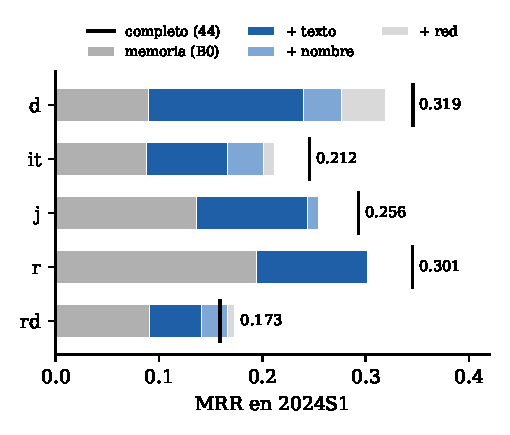
\includegraphics[width=\columnwidth]{figuras/escalera.pdf}
\caption{MRR por rubro al incorporar sucesivamente texto, nombre y red a la memoria. Las líneas negras corresponden a la referencia de 44 pistas sin selección lasso.}
\label{fig:escalera}
\end{figure}

El modelo lasso controla la complejidad mediante una penalización: al aumentar un parámetro $\lambda$, algunos coeficientes quedan exactamente en cero. El camino de regularización (\cref{fig:camino}) muestra que cinco pistas de memoria, texto y nombre alcanzan un MRR de validación de $0{,}238$; con 17 pistas, que ya incluyen la red, aumenta a $0{,}284$, y el modelo seleccionado llega a $0{,}308$. Las pistas adicionales mejoran el ranking, pero corresponden mayormente a variantes de las mismas cuatro ideas.

\begin{figure}[t]
\centering
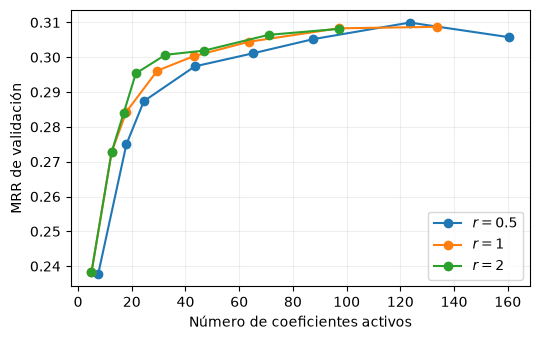
\includegraphics[width=\columnwidth]{figuras/output.png}
\caption{MRR de validación en función del número de coeficientes no nulos. Las curvas comparan penalizaciones relativas distintas para correcciones por rubro.}
\label{fig:camino}
\end{figure}

\paragraph{Rubro.} Se ensayaron coeficientes $\beta_{k,v}=\mu_k+\delta_{k,v}$, con una corrección específica para cada rubro $v$. El tronco solo y el modelo con correcciones alcanzaron prácticamente el mismo MRR promedio ($0{,}282$); al excluir un rubro del entrenamiento, el promedio descendió a $0{,}273$ (\cref{tab:mrr}), con diferencias que varían entre rubros. 

\paragraph{Modelos nulos.} Para evaluar la contribución de las distintas fuentes de información, se comparó el modelo original con cuatro escenarios de control (\cref{fig:nulos}): la exclusión de las pistas textuales, la permutación de las descripciones históricas y los perfiles empresariales (\emph{empresas falsas}), la asignación aleatoria de ganadores a las licitaciones (\emph{ganadores barajados}) y el modelo de referencia B0. Los dos controles de aleatorización permiten evaluar si el rendimiento depende de asociaciones reales entre los datos, al destruirlas mediante permutaciones aleatorias. En particular, el control de empresas falsas reduce el MRR entre $0{,}06$ y $0{,}10$ en d, it, j y r, sin diferencias significativas en rd. Dado que este control también modifica la preselección de candidatas, su efecto comprende tanto la recuperación como el reordenamiento.

\begin{figure}[t]
\centering
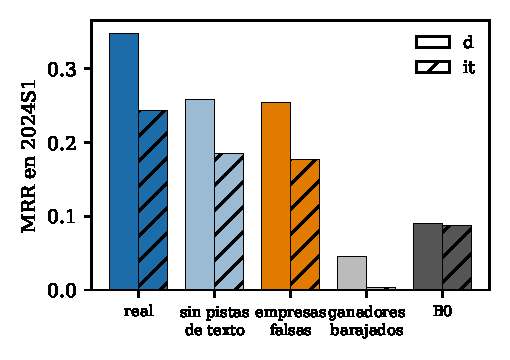
\includegraphics[width=\columnwidth]{figuras/nulos_falsas.pdf}
\caption{Comparación del MRR para el modelo original (real), la exclusión de pistas textuales, dos controles de aleatorización y el baseline B0, en los rubros d e it.}
\label{fig:nulos}
\end{figure}

El modelo propuesto es transferible, es decir, con una sola fórmula rinde lo mismo o más que modelos entrenados rubro por rubro. Además, cada parte se puede verificar: cada peso tiene un significado, y cada idea sobrevive a un modelo nulo. Finalmente compite con métodos mucho más complejos. LambdaMART, un método estándar de la industria que combina cientos de árboles de decisión \cite{burges2010} logró un MRR apenas mayor en dos rubros (j y r) y uno menor en it. Con las mismas pistas, los dos métodos no se distinguieron significativamente, de modo que el resultado depende sobre todo de qué información se le da al modelo.

%\section{Declaración de uso de IA}
%En este trabajo se utilizaron agentes de inteligencia artificial tales como Claude (Anthropic) y Chat GPT (Open AI) para la búsqueda de papers y referencias utilizadas en el mismo. Se contó con dichos asistentes para la optimización del código aplicado en las soluciones y para corregir la ortografía y gramática del presente informe. 

\balance
\section{Conclusión}

Un modelo de Boltzmann lineal en la energía permite integrar información heterogénea en coeficientes interpretables, y el lasso selecciona variantes útiles sin abandonar la estructura física. El texto aporta la mayor mejora sobre B0, seguido por la mención de nombres específicos; la red resulta relevante en determinados rubros. Su buen desempeño sin correcciones por rubro sugiere que estas relaciones se transfieren entre sectores.


La principal limitación es la cobertura, cuando ningún ganador ingresa al pool, el modelo no puede priorizarlo mediante las pistas. Además, la prueba 2024S1 fue consultada en otras exploraciones del proyecto, por lo que su resultado puede ser optimista \cite{cawley2010}. 
%La evaluación definitiva requiere licitaciones posteriores; otra dirección es mejorar la recuperación inicial de empresas poco representadas en el historial.
